\documentclass{beamer}
\usetheme{Copenhagen}
\usecolortheme{seahorse}

\usepackage{tikz}
\usepackage{graphicx}
\usepackage{listings}
\usepackage{xcolor}
\usepackage{hyperref}
\usepackage{esdiff}

\graphicspath{ {../images/} }

\title{A Random Model of the Primes}
\author{Frank Qiang, Aravinth Venkatesh Natarajan, Anthony Hong}
\institute{Georgia Institute of Technology}
\date{April 25, 2023}

\begin{document}
\frame{\titlepage}
\begin{frame}{Background}
  \begin{itemize}
    \item Infinite number of primes (c. 300 BC, Euclid)
    \item $\pi(x) := \text{number of primes} \leq x$
    \item Prime number theorem: $\pi(x) \sim \frac{x}{\ln x}$ (1896, Hadamard and De la Vall\'ee Poussin)
  \end{itemize}
\end{frame}

\begin{frame}{Prime Gaps}
  \begin{itemize}
    \item Prime gap := difference between a pair of consecutive primes
    \item What does the sequence of prime gaps look like?
      \[[1,2,2,4,2,4,2,4,6,2]\]
      Notice that 1 is the only odd.
    \item How small/large can prime gaps get?
    \begin{itemize}
      \item Small: twin prime conjecture; we have a constant bound by Yitang Zhang (2013), since improved to gap
        $\le 246$ infinitely often
      \item Large: can find gaps of arbitary size (think $n!$); so slightly different goal, want to see how large of a gap we can expect in a given interval
    \end{itemize}
  \end{itemize}
\end{frame}

\begin{frame}{Cramer's Random Model}
  \begin{itemize}
    \item We know prime number distribution isn't exactly random, but it seems to behave that way: try to model as if it were
    \item In the interval $[2, n]$, we expect roughly $\frac{n}{\ln n}$ primes by prime number theorem. There are also roughly $n$ total numbers $[2, n]$. So $n$ has probability $\frac{1}{\ln n}$ of being prime?
    \item Naively assign each $x \in \mathbb{N}_{>2}$ a probability of $\frac{1}{\ln x}$ of being prime
  \end{itemize}
\end{frame}

\begin{frame}{First Iteration}
  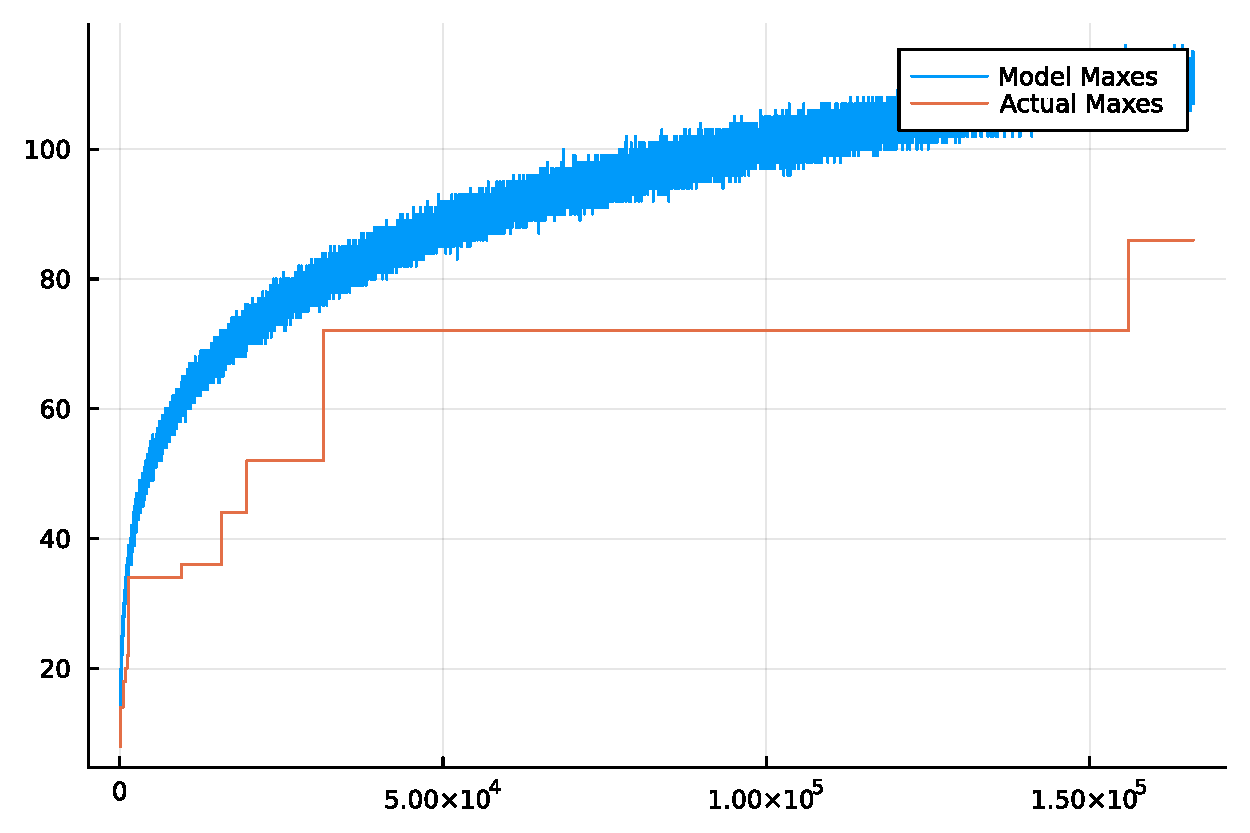
\includegraphics[width=\textwidth]{random-plot1.pdf}

  Plot of estimated largest gap $\le n$ vs. $n$, with
  100 trials per $n$.
\end{frame}

\begin{frame}{Why?}
  \begin{itemize}
    \item We can study this random distribution using ideas from probability and statistics, can give extra insight
    \item Conducting many trials comes at relatively low cost (can be parallelized, will scale with current trend towards multithreaded computers)
    \item We can consider disjoint intervals completely independently (not true of traditional sieve methods)
  \end{itemize}
\end{frame}
\begin{frame}{Improvement to the Original Model}
  \begin{itemize}
      \item Something obvious, the only even prime should be 2
      \item However, Cramer's original scheme gives all natural numbers $x > 2$ chance $\frac{1}{\ln{x}}$
      \item Idea: For every even number $e$, give its chance to $e + 1$
      \item Even number, $p(x) = 0$, odd number, $p(x) \approx \frac{2}{\ln{x}}$
  \end{itemize}
\end{frame}
\begin{frame}{Improvement to the Original Model}
    \begin{itemize}
        \item Extrapolate idea: Instead of just 2, consider a small prefix of primes
        \item Only consider numbers coprime to those primes to be a part of the model
        \item Maintains randomness, but incorporates some structure from that prefix
    \end{itemize}
\end{frame}
\begin{frame}
    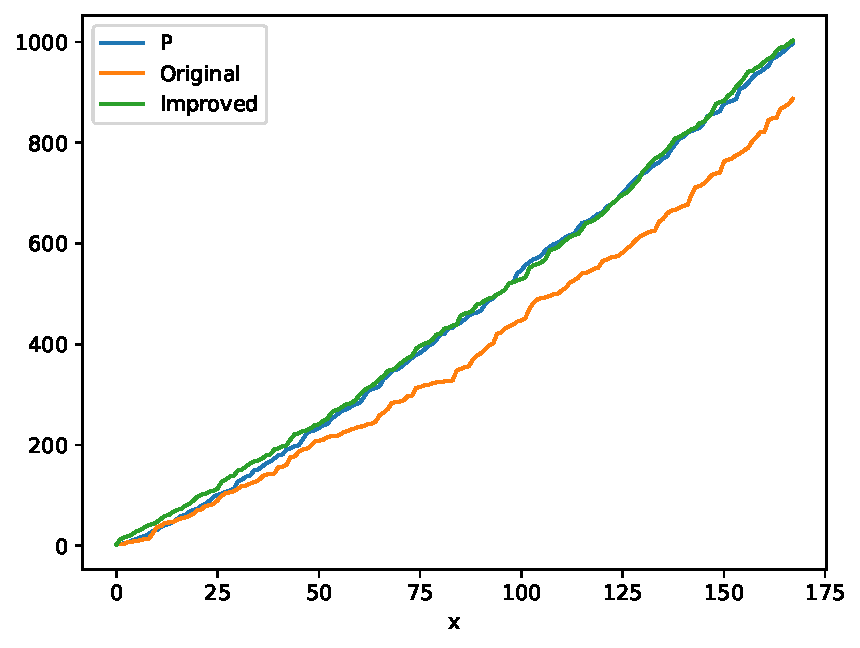
\includegraphics[width=\textwidth]{../images/Improvement.pdf}
\end{frame}
\begin{frame}{Extension of Cramer's Model}
    \begin{itemize}
        \item Cramer's model can be applied to other seemingly random sequences with known density
        \item e.g. Ulam numbers
        \item $U(1) = 1, U(2) = 2$
        \item $U(x)$ is least number which is a unique sum of two distinct earlier terms
    \end{itemize}
\end{frame}
\begin{frame}{Primes Themselves}
\begin{itemize}
    \item Fermat's Little Theorem, $a^{n - 1} \equiv 1 \mod n \; \forall a$ coprime to n 
    \item But, how accurate is this?
    \item Rewrite $n - 1 = 2^s d$
    \item $a^d \equiv 1 \pmod{n}$
    \item $a^{2^r d} \equiv -1 \pmod{n}, \quad 0 \leq r < s.$
\end{itemize}
\end{frame}
\begin{frame}{Miller Rabin}
\begin{itemize}
    \item No non-prime, odd, number exists that can pass for every a!!
    \item If the a chosen reveals that n is composite, it is called a witness. If it turns out it told us that a composite was prime, we call it a liar
    \item We don't know any way to deterministically find witnesses for a number
    \item So... Randomize!!
    \item It is shown that for 2 $<$ a $<$ n - 1, there are at most (1/4) * n liars
\end{itemize}
\end{frame}
\begin{frame}{Miller-Rabin}
    \begin{itemize}
        \item Doing k iterations of the algorithm, we have a confidence of $0.25^{k}$ that the number is prime
        \item In reality, the number of liars is much higher for most numbers
        \item This produces something known as an 'industry-grade' prime
        \item The running time is incredibly fast. The next slide will show Miller-Rabin in comparison with other algorithms
    \end{itemize}
\end{frame}
\begin{frame}{Running Time}
      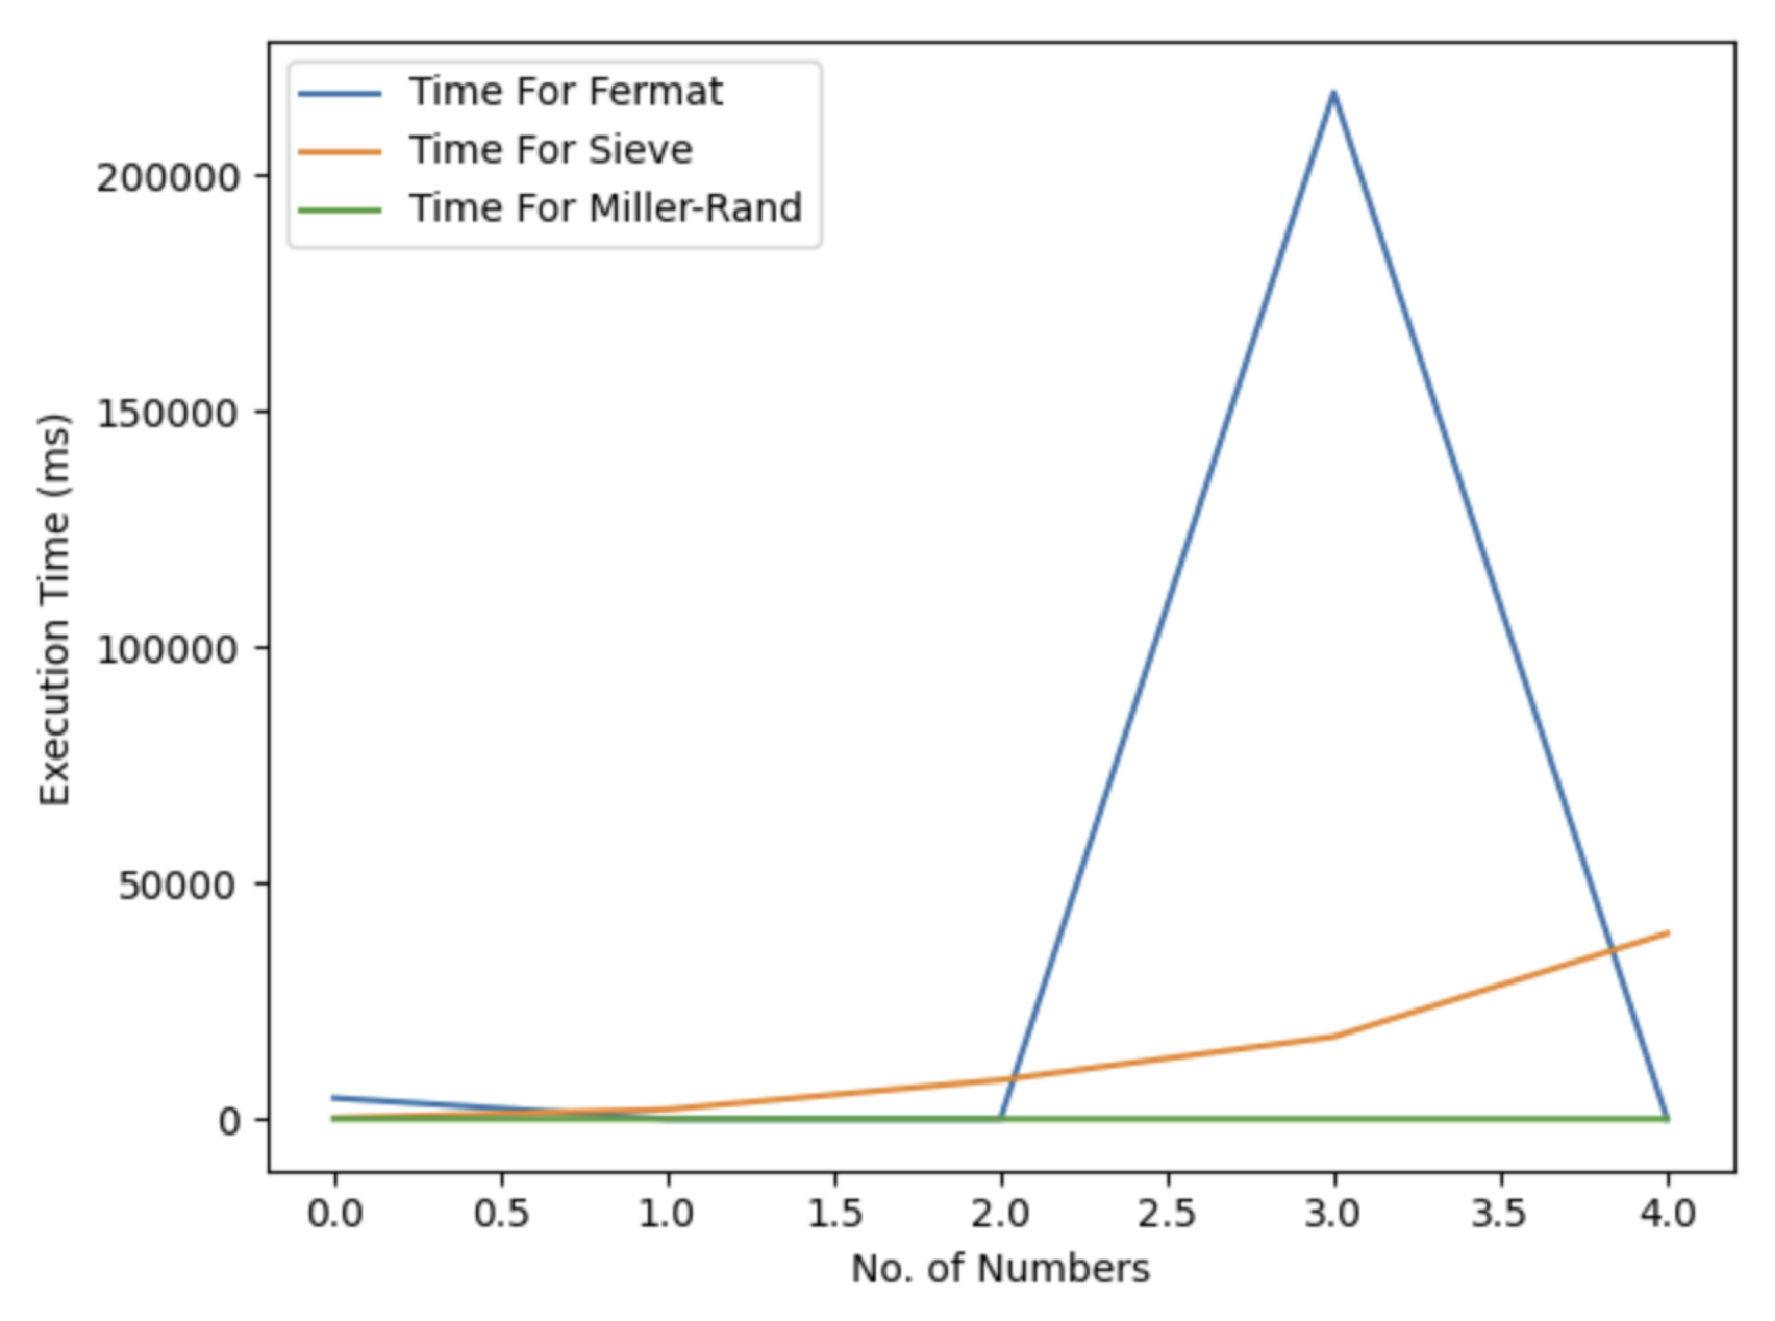
\includegraphics[width=\textwidth]{Fermat-Sieve-MillerRand.pdf}
\end{frame}
\begin{frame}{Running Time}
      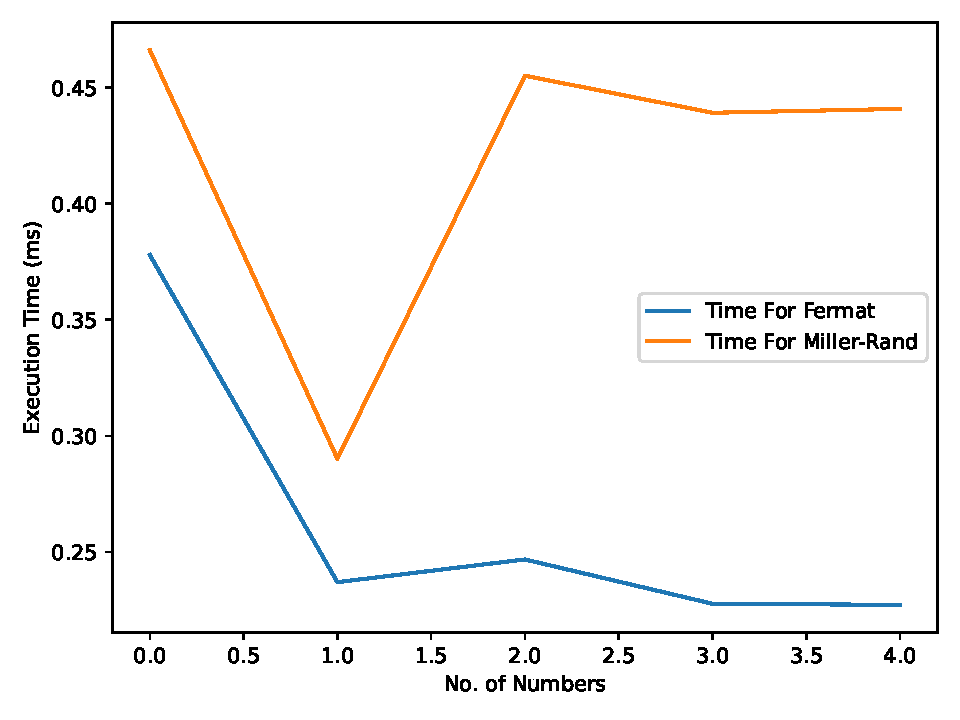
\includegraphics[width=\textwidth]{Fermat-MillerRand.pdf}
\end{frame}
\begin{frame}{Other Primality tests}
    \begin{itemize}
        \item The $\textbf{The Baillie-PSW}$ primality test is one that is possibly deterministic
        \item It is a mix between a Miller-Rabin test with a = 2(chosen arbitrarily) and another class of numbers called Lucas primes
        \item There is no known crossover between the two sets of numbers upto $2^{64}$
        
\includegraphics[width=\textwidth]{PepeSweat.pdf}
    \end{itemize}
\end{frame}
\end{document}
